%%%%%%%%%%%%%%%%%%%%%%%%%%%%%%%%%%%%%%%%%%%%%%%%%%%%%%%%%%%%%%%%%%%%%%%%%%%%%%%%%%%%%%%%%%%%%%%%
%
% CSCI 1430 Written Question Template
%
% This is a LaTeX document. LaTeX is a markup language for producing documents.
% Your task is to answer the questions by filling out this document, then to
% compile this into a PDF document.
% You will then upload this PDF to `Gradescope' - the grading system that we will use.
% Instructions for upload will follow soon.
%
%
% TO COMPILE:
% > pdflatex thisfile.tex
%
% If you do not have LaTeX and need a LaTeX distribution:
% - Departmental machines have one installed.
% - Personal laptops (all common OS): http://www.latex-project.org/get/
%
% If you need help with LaTeX, come to office hours. Or, there is plenty of help online:
% https://en.wikibooks.org/wiki/LaTeX
%
% Good luck!
% James and the 1430 staff
%
%%%%%%%%%%%%%%%%%%%%%%%%%%%%%%%%%%%%%%%%%%%%%%%%%%%%%%%%%%%%%%%%%%%%%%%%%%%%%%%%%%%%%%%%%%%%%%%%
%
% How to include two graphics on the same line:
%
% \includegraphics[width=0.49\linewidth]{yourgraphic1.png}
% \includegraphics[width=0.49\linewidth]{yourgraphic2.png}
%
% How to include equations:
%
% \begin{equation}
% y = mx+c
% \end{equation}
%
%%%%%%%%%%%%%%%%%%%%%%%%%%%%%%%%%%%%%%%%%%%%%%%%%%%%%%%%%%%%%%%%%%%%%%%%%%%%%%%%%%%%%%%%%%%%%%%%

\documentclass[11pt]{article}

\usepackage[english]{babel}
\usepackage[utf8]{inputenc}
\usepackage{amssymb}

\usepackage[colorlinks = true,
            linkcolor = blue,
            urlcolor  = blue]{hyperref}
\usepackage[a4paper,margin=1.5in]{geometry}
\usepackage{stackengine,graphicx}
\usepackage{fancyhdr}
\setlength{\headheight}{15pt}
\usepackage{microtype}
\usepackage{times}
\usepackage[shortlabels]{enumitem}
\setlist[enumerate]{topsep=0pt}
\usepackage{amsmath}

% a great python code format: https://github.com/olivierverdier/python-latex-highlighting
\usepackage{pythonhighlight}

\frenchspacing
\setlength{\parindent}{0cm} % Default is 15pt.
\setlength{\parskip}{0.3cm plus1mm minus1mm}

\pagestyle{fancy}
\fancyhf{}
\lhead{Project 1 Questions}
\rhead{CSCI 1430}
\rfoot{\thepage}

\date{}

\title{\vspace{-1cm}Project 1 Questions}


\begin{document}
\maketitle
\vspace{-3cm}
\thispagestyle{fancy}

\section*{Instructions}
\begin{itemize}
  \item 5 questions.
  \item Include code, images, and equations where appropriate.
  \item Please make this document anonymous.
  \item When you are finished, compile this document to a PDF and submit it directly to Gradescope. On upload, \textbf{Gradescope will ask you to assign question numbers to your pages}. Making each question end with a page break after your answer is a good way to ease this process.
\end{itemize}

\section*{Questions}

\paragraph{Q1:} Image convolution, a type of image filtering, is a fundamental image processing tool that you will use repeatedly throughout the course.

\begin{enumerate}[(a)]
\item \emph{Explicitly describe} the 3 main components of image convolution:
\begin{enumerate}[(i)]
    \item input
    \item transformation (how it happens)
    \item output
\end{enumerate}
\item Why is image convolution important in Computer Vision? Which applications does it allow?
\end{enumerate}


%%%%%%%%%%%%%%%%%%%%%%%%%%%%%%%%%%%
\paragraph{A1:} Your answer here.
% Uncomment the stencil below and fill in your solution.

% \begin{enumerate}[(a)]
% \item 
% \begin{enumerate}[(i)]
%     \item 
%     \item
%     \item 
% \end{enumerate}
% \item 
% \end{enumerate}

%%%%%%%%%%%%%%%%%%%%%%%%%%%%%%%%%%%

% Please leave the pagebreak
\pagebreak
\paragraph{Q2:} Correlation is another basic image operation. Correlation and convolution are, in some sense, the simplest operations we can perform to extract information from images.
\begin{enumerate}[(a)]
    \item 
    What is the difference between convolution and correlation?

    \item
    Construct a scenario which produces a different output between both operations. Include the kernel you used and your image results.
    
    \emph{Please use \href{https://docs.scipy.org/doc/scipy/reference/generated/scipy.ndimage.convolve.html}{$scipy.ndimage.convolve$} and \href{https://docs.scipy.org/doc/scipy/reference/generated/scipy.ndimage.correlate.html}{$scipy.ndimage.correlate$} to experiment!}
    
\end{enumerate}


%%%%%%%%%%%%%%%%%%%%%%%%%%%%%%%%%%%
\paragraph{A2:} Your answer here.
% Uncomment the stencil below and fill in your solution.

% \begin{enumerate}[(a)]

% \item 

% \item 

% \end{enumerate}

%%%%%%%%%%%%%%%%%%%%%%%%%%%%%%%%%%%

% Please leave the pagebreak
\pagebreak
\paragraph{Q3:} We create hybrid images by high pass filtering one image, low pass filtering another image, and summing the two images. For (a--c), which filter does the kernel represent? For (d--e), which filter produced the output images?

%%%%%%%%%%%%%%%%%%%%%%%%%%%%%%%%%%%
\emph{LaTeX:} To fill in boxes, replace `\textbackslash square' with `\textbackslash blacksquare' for your answer.

\begin{enumerate}[(a)]
\item
 $\begin{bmatrix}
    1 & 0 & -1 \\
    1 & 0 & -1 \\
    1 & 0 & -1 \\
 \end{bmatrix}$
\begin{tabular}[h]{ll}
$\square$ & High pass \\
$\square$ & Low pass \\
$\square$ & Neither \\
\end{tabular}

\item
 $\begin{bmatrix}
    \frac{1}{9} & \frac{1}{9} & \frac{1}{9} \\
    \frac{1}{9} & \frac{1}{9} & \frac{1}{9} \\
    \frac{1}{9} & \frac{1}{9} & \frac{1}{9}
 \end{bmatrix}$
\begin{tabular}[h]{ll}
$\square$ & High pass \\
$\square$ & Low pass \\
$\square$ & Neither \\
\end{tabular}

\item
$\begin{bmatrix}
    -\frac{1}{9} & -\frac{1}{9} & -\frac{1}{9} \\
    -\frac{1}{9} & \frac{8}{9} & -\frac{1}{9} \\
    -\frac{1}{9} & -\frac{1}{9} & -\frac{1}{9}
  \end{bmatrix}$
\begin{tabular}[h]{ll}
$\square$ & High pass \\
$\square$ & Low pass \\
$\square$ & Neither \\
\end{tabular}

\item
Input image:\\
\raisebox{\baselineskip-\height}{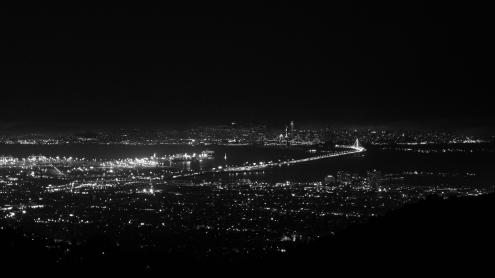
\includegraphics[width = 6cm]{q3img0.png}} \\
Output image 1:\\
\raisebox{\baselineskip-\height}{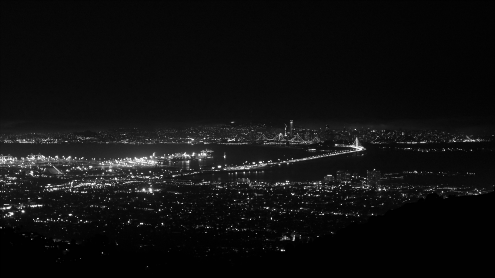
\includegraphics[width = 6cm]{q3img1.png}}
\begin{tabular}[h]{lc}
$\square$ & High pass \\
$\square$ & Low pass \\
\end{tabular}

\item
Output image 2:\\
\raisebox{\baselineskip-\height}{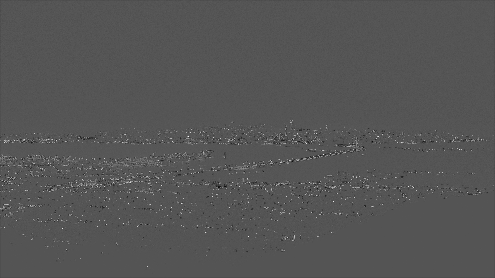
\includegraphics[width = 6cm]{q3img2.png}}
\begin{tabular}[h]{lc}
$\square$ & High pass \\
$\square$ & Low pass \\
\end{tabular}

\item
Which of the following statements are true? (Check all that apply).

\begin{tabular}[h]{ll}
$\square$ & High pass filter kernels will always contain at least one negative number \\
$\square$ & A Gaussian filter is an example of a low pass filter \\
$\square$ & A high pass filter is the basis for most smoothing methods \\
$\square$ & In a high pass filter, the center of the kernel must have the highest value \\
\end{tabular}

\end{enumerate}



%%%%%%%%%%%%%%%%%%%%%%%%%%%%%%%%%%%

% Please leave the pagebreak
\pagebreak
\paragraph{Q4:} 
\begin{enumerate}[(a)]
    \item 
How does computation time vary with filter sizes from $3\times3$ to $15\times15$ (test odd and square sizes, i.e. $3\times3$, $5\times5$, $7\times7$, etc.), and with image sizes from approximately 0.25 to 8 megapixels. Choose your own intervals.

\emph{A megapixel is 1,048,576 ($2^20$) pixels (1024$\times$1024), or sometimes also 1,000,000 pixels (especially if you manufacture cameras). Megapixels is often shortened to MP or MPix.}

Measure both using \href{https://docs.scipy.org/doc/scipy/reference/generated/scipy.ndimage.convolve.html}{$scipy.ndimage.convolve$} or \href{https://docs.scipy.org/doc/scipy/reference/generated/scipy.ndimage.correlate.html}{$scipy.ndimage.correlate$} to produce a set of values. Use the \href{http://scikit-image.org/docs/dev/auto_examples/transform/plot_rescale.html}{$skimage.transform$} module with its {$rescale$} function to vary the size of an image. Use an appropriate charting function to plot your matrix of results, e.g., by plotting multiple lines on a graph using \href{https://matplotlib.org/api/_as_gen/matplotlib.pyplot.plot.html}{$Plot$}, with one for each kernel size.

\emph{Image:} \href{RISDance.jpg}{RISDance.jpg} (in the .tex directory).

\item
    Do the results match your expectation given the number of multiply and add operations in convolution?
\end{enumerate}

%%%%%%%%%%%%%%%%%%%%%%%%%%%%%%%%%%%
\paragraph{A4:} Your answer here.
% Uncomment the stencil below and fill in your solution.

% \begin{enumerate}[(a)]

% \item 

% \item 

% \end{enumerate}

%%%%%%%%%%%%%%%%%%%%%%%%%%%%%%%%%%%


% Please leave the pagebreak
\pagebreak
\paragraph{Q5:} 
In 1990, \emph{New York Times} photography critic Andy Grundberg \href{https://www.nytimes.com/1990/08/12/arts/photography-view-ask-it-no-questions-the-camera-can-lie.html}{stated that:}\\``In the future, readers of newspapers and
magazines will probably view news pictures more as
illustrations than as reportage, since they can no longer distinguish between a genuine image and one that has been manipulated.''

\begin{enumerate}[(a)]
    \item When is Grundberg's `future' ? Why? (2--4 sentences)
    
    \item When is a news picture no longer genuine? Are any manipulations permissible, and if so, which ones? (2--4 sentences)
    
    \item If you worked for the \emph{New York Times} and were tasked with maintaining readers' trust in news pictures in Grundberg's future, what would you do? Consider everything that happens in the publication of a news picture. Describe your approach, and why it would work. (3--5 sentences)
    
    \begin{enumerate}[(i)]
    \item As per c), but instead you worked for the \emph{College Hill Independent}? \\(2--4 sentences)
    \end{enumerate}
    
    \item Include an cited example of a manipulated news picture, and identify the manipulation. What was the intent and impact of the manipulation? (2--4 sentences)
\end{enumerate}

\emph{Note:} There are open questions. We will grade for thought and justification. 

%%%%%%%%%%%%%%%%%%%%%%%%%%%%%%%%%%%
\paragraph{A5:} Your answer here.
% Uncomment the stencil below and fill in your solution.

% \begin{enumerate}[(a)]

% \item 

% \item 
% \item Answer here. 
% \begin{enumerate}[(i)]
%     \item Answer here.
% \end{enumerate}

% \item 

% \end{enumerate}

%%%%%%%%%%%%%%%%%%%%%%%%%%%%%%%%%%%

\pagebreak
\paragraph{A5:} Continued; extra space as needed.


\pagebreak
\section*{Feedback? (Optional)}
Please help us make the course better. If you have any feedback for this assignment, we'd love to hear it!

%%%%%%%%%%%%%%%%%%%%%%%%%%%%%%%%%%%


\end{document}